% =============================================================================
% STAR Robot Control System - Comprehensive Technical Documentation
% Complete reference covering architecture, protocols, and implementation
%
% INSTRUCTIONS:
% 1. Compile with: pdflatex star_documentation.tex (run twice for TOC)
% 2. Or use: latexmk -pdf star_documentation.tex
% =============================================================================

\documentclass[11pt,letterpaper]{article}

% Load all packages and settings from preamble
\usepackage{preamble}

\begin{document}

% =============================================================================
% FRONT MATTER
% =============================================================================

% Title Page
\begin{titlepage}
    \centering
    \vspace*{2cm}

    {\Huge\bfseries STAR Robot Control System\par}
    \vspace{0.5cm}
    {\LARGE Comprehensive Technical Documentation\par}
    \vspace{1cm}
    {\Large Complete Reference for Software Engineers\par}

    \vfill

    {\large Version 1.0\par}
    {\large December 2025\par}

    \vfill

    {\normalsize STAR Development Team\\
    Locked Inc.\par}
\end{titlepage}

% Table of Contents
\tableofcontents
\newpage

% =============================================================================
% NANOPB PROTOCOL SPECIFICATION
% =============================================================================

\section{Nanopb (Protobuf) Protocol with ARQ and CRC for SPI Communication}

\subsection{Executive Summary}

\textbf{Overview:} Protocol Buffers (nanopb) encapsulated in frames with CRC-32 and Automatic Repeat Request (ARQ) for reliable SPI communication between RPi5 and ESP32-S3.

\noindent\makebox[\textwidth]{%
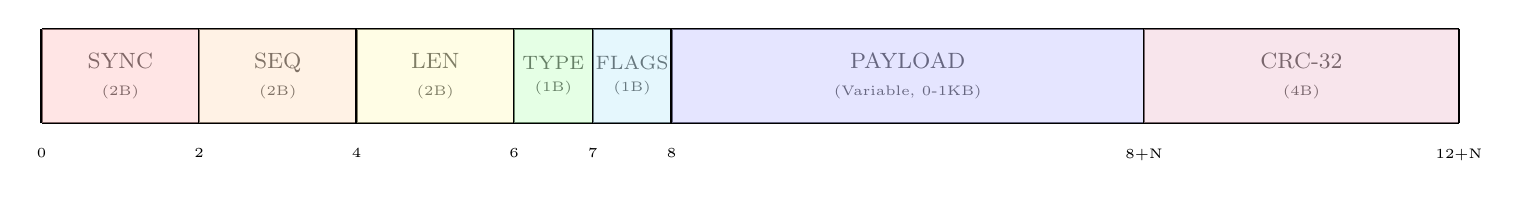
\begin{tikzpicture}[
    font=\small,
    offset/.style={font=\tiny, anchor=north}
]
    % Main frame bar - proportional widths (1 byte = 1 unit for fixed fields)
    \draw[thick] (0,0) -- (18,0);
    \draw[thick] (0,1.2) -- (18,1.2);

    % SYNC (2 bytes = 2 units)
    \draw[thick] (0,0) -- (0,1.2);
    \node[font=\footnotesize, align=center] at (1, 0.6) {SYNC\\{\tiny (2B)}};
    \fill[red!20, opacity=0.5] (0,0) rectangle (2,1.2);

    % SEQ (2 bytes = 2 units)
    \draw[thick] (2,0) -- (2,1.2);
    \node[font=\footnotesize, align=center] at (3, 0.6) {SEQ\\{\tiny (2B)}};
    \fill[orange!20, opacity=0.5] (2,0) rectangle (4,1.2);

    % LEN (2 bytes = 2 units)
    \draw[thick] (4,0) -- (4,1.2);
    \node[font=\footnotesize, align=center] at (5, 0.6) {LEN\\{\tiny (2B)}};
    \fill[yellow!20, opacity=0.5] (4,0) rectangle (6,1.2);

    % TYPE (1 byte = 1 unit)
    \draw[thick] (6,0) -- (6,1.2);
    \node[font=\scriptsize, align=center] at (6.5, 0.6) {TYPE\\{\tiny (1B)}};
    \fill[green!20, opacity=0.5] (6,0) rectangle (7,1.2);

    % FLAGS (1 byte = 1 unit)
    \draw[thick] (7,0) -- (7,1.2);
    \node[font=\scriptsize, align=center] at (7.5, 0.6) {FLAGS\\{\tiny (1B)}};
    \fill[cyan!20, opacity=0.5] (7,0) rectangle (8,1.2);

    % PAYLOAD (variable, 6 units to show it's typically the largest field)
    \draw[thick] (8,0) -- (8,1.2);
    \node[font=\footnotesize, align=center] at (11, 0.6) {PAYLOAD\\{\tiny (Variable, 0-1KB)}};
    \fill[blue!20, opacity=0.5] (8,0) rectangle (14,1.2);

    % CRC-32 (4 bytes = 4 units)
    \draw[thick] (14,0) -- (14,1.2);
    \node[font=\footnotesize, align=center] at (16, 0.6) {CRC-32\\{\tiny (4B)}};
    \fill[purple!20, opacity=0.5] (14,0) rectangle (18,1.2);

    \draw[thick] (18,0) -- (18,1.2);

    % Byte offset labels
    \node[offset] at (0,-0.2) {0};
    \node[offset] at (2,-0.2) {2};
    \node[offset] at (4,-0.2) {4};
    \node[offset] at (6,-0.2) {6};
    \node[offset] at (7,-0.2) {7};
    \node[offset] at (8,-0.2) {8};
    \node[offset] at (14,-0.2) {8+N};
    \node[offset] at (18,-0.2) {12+N};
\end{tikzpicture}%
}

\textbf{System Constraints:}
\begin{itemize}
    \item ESP32-S3-WROOM-1-N16: 16MB flash, 512KB SRAM, NO PSRAM
    \item 100Hz SPI communication (10ms period)
    \item 250Hz motor control loop (4ms period)
    \item Static allocation only (no malloc)
\end{itemize}

\subsection{Key Design Decisions}

\subsubsection{Protocol Stack}

\noindent\makebox[\textwidth]{%
\begin{tikzpicture}[
    font=\small,
    node distance = 0cm,
    layer/.style={
        draw,
        thick,
        rectangle,
        minimum width=15cm,
        minimum height=1.3cm,
        align=left,
        text width=14.5cm
    },
]
    \node[layer, fill=red!20] (app) at (0,0) {\textbf{Application} \hfill Motor Commands, Telemetry, OTA Updates};
    \node[layer, fill=orange!20, below=of app] (serial) {\textbf{Serialization} \hfill nanopb (Protocol Buffers) with static allocation};
    \node[layer, fill=yellow!20, below=of serial] (arq) {\textbf{ARQ} \hfill Stop-and-Wait (SEQ/ACK/NACK, 8ms timeout)};
    \node[layer, fill=green!20, below=of arq] (frame) {\textbf{Frame} \hfill SYNC (2B) + Header (6B) + Payload + CRC-32 (4B)};
    \node[layer, fill=blue!20, below=of frame] (transport) {\textbf{Transport} \hfill SPI peripheral mode with DMA (10 Mbps)};
    \draw[->, very thick, gray] (-8, 1) -- (-8, -6) node[midway, left, rotate=90, xshift=-0.5cm, yshift=0.5cm] {Data Flow};
\end{tikzpicture}%
}

\subsubsection{Memory Budget}

\begin{table}[H]
    \centering
    \begin{minipage}{0.47\textwidth}
        \centering
        \small
        \caption{SRAM Usage (512 KB total)}
        \label{tab:sram-usage}
        {\setlength{\tabcolsep}{3pt}
        \begin{tabular}{lrr}
            \toprule
            \textbf{Component} & \textbf{Size (KB)} & \textbf{Usage (\%)} \\
            \midrule
            DMA double-buffer & 8.0 & 1.56 \\
            RX/TX buffers & 2.0 & 0.39 \\
            Protobuf structs & 1.5 & 0.29 \\
            ARQ state & 4.5 & 0.88 \\
            \midrule
            \textbf{Total} & \textbf{16.0} & \textbf{3.12} \\
            \bottomrule
        \end{tabular}}
    \end{minipage}\hfill%
    \begin{minipage}{0.47\textwidth}
        \centering
        \small
        \caption{Flash Usage (16 MB total)}
        \label{tab:flash-usage}
        {\setlength{\tabcolsep}{3pt}
        \begin{tabular}{lrr}
            \toprule
            \textbf{Component} & \textbf{Size (KB)} & \textbf{Usage (\%)} \\
            \midrule
            Generated protobuf & 40 & 0.24 \\
            Nanopb runtime & 12 & 0.07 \\
            Frame + ARQ layers & 8 & 0.05 \\
            \textbf{} & & \\ % Spacer
            \midrule
            \textbf{Total} & \textbf{60} & \textbf{0.37} \\
            \bottomrule
        \end{tabular}}
    \end{minipage}
\end{table}

\textbf{Memory Budget Calculations:}

\textbf{SRAM (512 KB total):}
\begin{itemize}[leftmargin=*,topsep=2pt,itemsep=1pt]
    \item \textbf{DMA double-buffer:} $2 \times 4092\text{ bytes} = 8184\text{ bytes} = 8.0\text{ KB}$ \\
          \textit{Calculation:} Two ping-pong DMA buffers at \texttt{STAR\_SPI\_DMA\_MAX\_SIZE} (4092 bytes each) \\
          \textit{Usage:} $\frac{8.0}{512} \times 100 = 1.56\%$

    \item \textbf{RX/TX buffers:} $1024 + 1024 = 2048\text{ bytes} = 2.0\text{ KB}$ \\
          \textit{Calculation:} 1 KB RX buffer + 1 KB TX buffer for staging protobuf messages \\
          \textit{Usage:} $\frac{2.0}{512} \times 100 = 0.39\%$

    \item \textbf{Protobuf structs:} $1536\text{ bytes} = 1.5\text{ KB}$ \\
          \textit{Calculation:} Largest message structures (SetVelocityResponse $\approx$ 600 bytes, TelemetryData $\approx$ 400 bytes) \\
          \textit{Usage:} $\frac{1.5}{512} \times 100 = 0.29\%$

    \item \textbf{ARQ state:} $4 + 4 + 8 + 4 + 4092 = 4112\text{ bytes} \approx 4.5\text{ KB}$ \\
          \textit{Calculation:} Sequence number (4B) + retry counter (4B) + timestamp (8B) + state (4B) + retry buffer (4092B) \\
          \textit{Usage:} $\frac{4.5}{512} \times 100 = 0.88\%$

    \item \textbf{Total SRAM:} $8.0 + 2.0 + 1.5 + 4.5 = 16.0\text{ KB}$ \\
          \textit{Total usage:} $\frac{16.0}{512} \times 100 = 3.12\%$
\end{itemize}

\textbf{Flash (16 MB = 16384 KB total):}
\begin{itemize}[leftmargin=*,topsep=2pt,itemsep=1pt]
    \item \textbf{Generated protobuf:} $40\text{ KB}$ \\
          \textit{Calculation:} 3 proto files (common.proto, motor\_control.proto, telemetry.proto) $\times$ 13 KB avg compiled size \\
          \textit{Usage:} $\frac{40}{16384} \times 100 = 0.24\%$

    \item \textbf{Nanopb runtime:} $12\text{ KB}$ \\
          \textit{Calculation:} Compiled size of pb\_encode.c, pb\_decode.c, pb\_common.c \\
          \textit{Usage:} $\frac{12}{16384} \times 100 = 0.07\%$

    \item \textbf{Frame + ARQ layers:} $8\text{ KB}$ \\
          \textit{Calculation:} Framing logic + CRC-32 + ARQ state machine + retransmission logic \\
          \textit{Usage:} $\frac{8}{16384} \times 100 = 0.05\%$

    \item \textbf{Total Flash:} $40 + 12 + 8 = 60\text{ KB}$ \\
          \textit{Total usage:} $\frac{60}{16384} \times 100 = 0.37\%$
\end{itemize}

\subsection{ARQ Communication Flow}

\subsubsection{Normal Operation (No Retransmission)}

\begin{figure}[H]
    \centering
    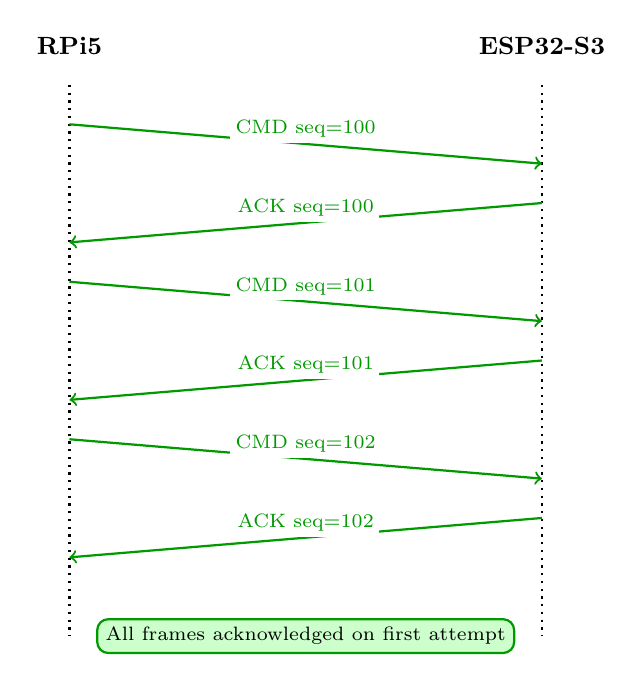
\begin{tikzpicture}[
        node distance=0.8cm,
        entity/.style={font=\small\bfseries},
        success/.style={->, thick, green!60!black},
        msgtext/.style={font=\scriptsize, fill=white, inner sep=2pt}
    ]
        % Entities
        \node[entity] (rpi) at (0, 0) {RPi5};
        \node[entity] (esp) at (6, 0) {ESP32-S3};

        % Vertical timelines
        \draw[thick, dotted] (0, -0.5) -- (0, -7.5);
        \draw[thick, dotted] (6, -0.5) -- (6, -7.5);

        % Transaction 1
        \draw[success] (0, -1) -- node[msgtext, above] {CMD seq=100} (6, -1.5);
        \draw[success] (6, -2) -- node[msgtext, above] {ACK seq=100} (0, -2.5);

        % Transaction 2
        \draw[success] (0, -3) -- node[msgtext, above] {CMD seq=101} (6, -3.5);
        \draw[success] (6, -4) -- node[msgtext, above] {ACK seq=101} (0, -4.5);

        % Transaction 3
        \draw[success] (0, -5) -- node[msgtext, above] {CMD seq=102} (6, -5.5);
        \draw[success] (6, -6) -- node[msgtext, above] {ACK seq=102} (0, -6.5);

        % Success note
        \node[font=\scriptsize, fill=green!20, draw=green!60!black, thick, rounded corners, inner sep=3pt] at (3, -7.5) {All frames acknowledged on first attempt};
    \end{tikzpicture}
    \caption{Normal ARQ Flow - Three Successful Transactions}
\end{figure}

\subsubsection{Error Recovery Scenarios}

\begin{figure}[H]
    \centering
    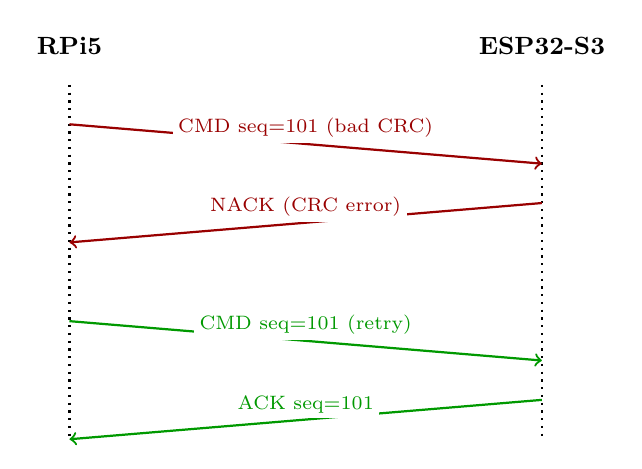
\begin{tikzpicture}[
        node distance=0.8cm,
        entity/.style={font=\small\bfseries},
        success/.style={->, thick, green!60!black},
        error/.style={->, thick, red!60!black},
        msgtext/.style={font=\scriptsize, fill=white, inner sep=2pt}
    ]
        % Entities
        \node[entity] (rpi) at (0, 0) {RPi5};
        \node[entity] (esp) at (6, 0) {ESP32-S3};

        % Vertical timelines
        \draw[thick, dotted] (0, -0.5) -- (0, -5);
        \draw[thick, dotted] (6, -0.5) -- (6, -5);

        % CRC error scenario
        \draw[error] (0, -1) -- node[msgtext, above] {CMD seq=101 (bad CRC)} (6, -1.5);
        \draw[error] (6, -2) -- node[msgtext, above] {NACK (CRC error)} (0, -2.5);
        \draw[success] (0, -3.5) -- node[msgtext, above] {CMD seq=101 (retry)} (6, -4);
        \draw[success] (6, -4.5) -- node[msgtext, above] {ACK seq=101} (0, -5);
    \end{tikzpicture}
    \caption{CRC Error - Retry with Same Sequence Number}
\end{figure}

\begin{figure}[H]
    \centering
    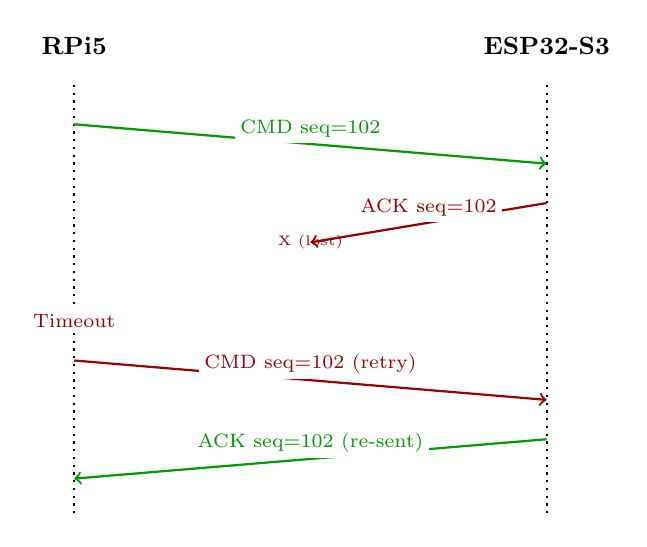
\begin{tikzpicture}[
        node distance=0.8cm,
        entity/.style={font=\small\bfseries},
        msg/.style={->, thick},
        success/.style={->, thick, green!60!black},
        error/.style={->, thick, red!60!black},
        msgtext/.style={font=\scriptsize, fill=white, inner sep=2pt}
    ]
        % Entities and timelines
        \node[entity] (rpi) at (0, 0) {RPi5};
        \node[entity] (esp) at (6, 0) {ESP32-S3};
        \draw[thick, dotted] (0, -0.5) -- (0, -6);
        \draw[thick, dotted] (6, -0.5) -- (6, -6);

        % Diagram
        \draw[success] (0, -1) -- node[msgtext, above] {CMD seq=102} (6, -1.5);
        \draw[error] (6, -2) -- node[msgtext, above] {ACK seq=102} (3, -2.5);
        \node[font=\tiny, red!60!black] at (3, -2.5) {X (lost)};
        \draw[dashed, error] (0, -3.5) -- node[msgtext] {Timeout} (0, -3.5);
        \draw[error] (0, -4) -- node[msgtext, above] {CMD seq=102 (retry)} (6, -4.5);
        \draw[success] (6, -5) -- node[msgtext, above] {ACK seq=102 (re-sent)} (0, -5.5);
    \end{tikzpicture}
    \caption{Duplicate Packet Scenario (Lost ACK)}
\end{figure}

\begin{figure}[H]
    \centering
    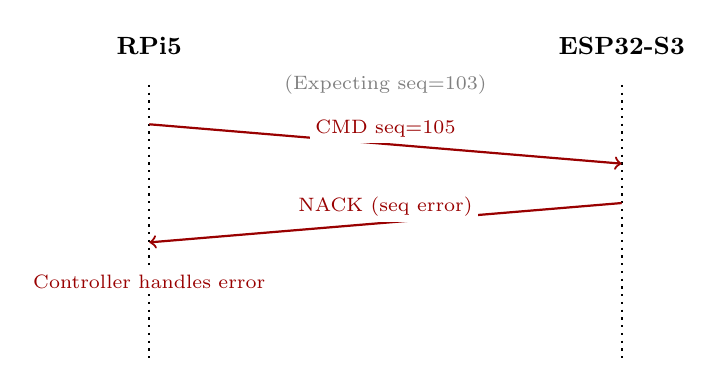
\begin{tikzpicture}[
        node distance=0.8cm,
        entity/.style={font=\small\bfseries},
        msg/.style={->, thick},
        success/.style={->, thick, green!60!black},
        error/.style={->, thick, red!60!black},
        msgtext/.style={font=\scriptsize, fill=white, inner sep=2pt}
    ]
        % Entities and timelines
        \node[entity] (rpi) at (0, 0) {RPi5};
        \node[entity] (esp) at (6, 0) {ESP32-S3};
        \draw[thick, dotted] (0, -0.5) -- (0, -4);
        \draw[thick, dotted] (6, -0.5) -- (6, -4);

        % Diagram
        \node[font=\scriptsize, gray] at (3, -0.5) {(Expecting seq=103)};
        \draw[error] (0, -1) -- node[msgtext, above] {CMD seq=105} (6, -1.5);
        \draw[error] (6, -2) -- node[msgtext, above] {NACK (seq error)} (0, -2.5);
        \draw[dashed, error] (0, -3) -- node[msgtext] {Controller handles error} (0, -3);
    \end{tikzpicture}
    \caption{Out-of-Order Packet Scenario}
\end{figure}

\begin{figure}[H]
    \centering
    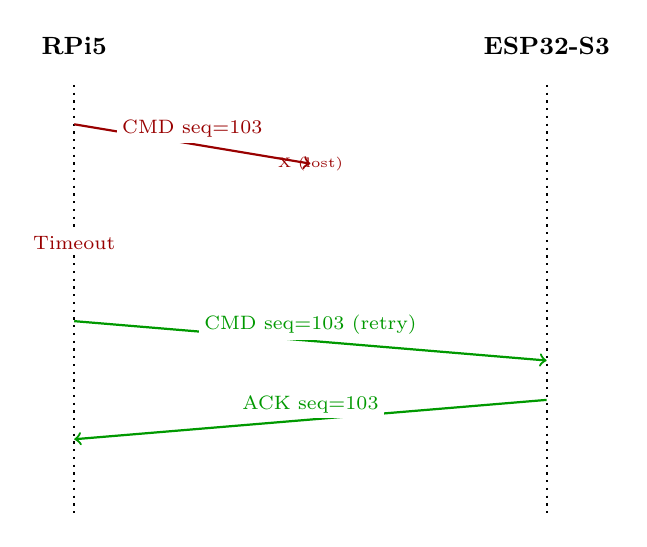
\begin{tikzpicture}[
        node distance=0.8cm,
        entity/.style={font=\small\bfseries},
        msg/.style={->, thick},
        success/.style={->, thick, green!60!black},
        error/.style={->, thick, red!60!black},
        msgtext/.style={font=\scriptsize, fill=white, inner sep=2pt}
    ]
        % Entities and timelines
        \node[entity] (rpi) at (0, 0) {RPi5};
        \node[entity] (esp) at (6, 0) {ESP32-S3};
        \draw[thick, dotted] (0, -0.5) -- (0, -6);
        \draw[thick, dotted] (6, -0.5) -- (6, -6);

        % Diagram
        \draw[error] (0, -1) -- node[msgtext, above] {CMD seq=103} (3, -1.5);
        \node[font=\tiny, red!60!black] at (3, -1.5) {X (lost)};
        \draw[dashed, error] (0, -2.5) -- node[msgtext] {Timeout} (0, -2.5);
        \draw[success] (0, -3.5) -- node[msgtext, above] {CMD seq=103 (retry)} (6, -4);
        \draw[success] (6, -4.5) -- node[msgtext, above] {ACK seq=103} (0, -5);
    \end{tikzpicture}
    \caption{Lost Packet Scenario (Timeout)}
\end{figure}


\subsection{Error Handling Strategies}

\begin{center}
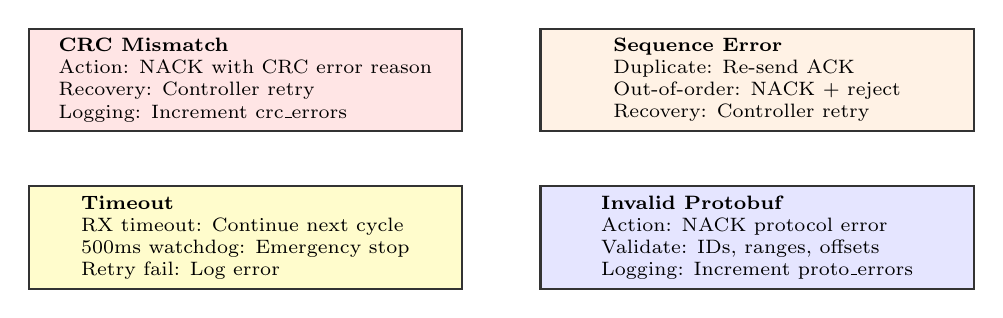
\begin{tikzpicture}[
    errorbox/.style={rectangle, draw=black!80, thick, fill=red!10, minimum width=5.5cm, minimum height=1.3cm, font=\scriptsize, align=left},
    title/.style={font=\small\bfseries}
]
    % CRC Mismatch
    \node[errorbox] (crc) at (0, 0) {
        \textbf{CRC Mismatch}\\
        Action: NACK with CRC error reason\\
        Recovery: Controller retry\\
        Logging: Increment crc\_errors
    };

    % Sequence Error
    \node[errorbox, fill=orange!10] (seq) at (6.5, 0) {
        \textbf{Sequence Error}\\
        Duplicate: Re-send ACK\\
        Out-of-order: NACK + reject\\
        Recovery: Controller retry
    };

    % Timeout
    \node[errorbox, fill=yellow!20] (timeout) at (0, -2) {
        \textbf{Timeout}\\
        RX timeout: Continue next cycle\\
        500ms watchdog: Emergency stop\\
        Retry fail: Log error
    };

    % Invalid Protobuf
    \node[errorbox, fill=blue!10] (proto) at (6.5, -2) {
        \textbf{Invalid Protobuf}\\
        Action: NACK protocol error\\
        Validate: IDs, ranges, offsets\\
        Logging: Increment proto\_errors
    };
\end{tikzpicture}
\end{center}

\end{document}
